\scanpage{107}
\mspage{98}
% archive sheet number: 107

En d'autres termes, on a \unsure{trouvé} une relation d'ordre sur $\unsure{\mathscr{M}|\mathcal{M}}$, telle que la relation $X\mathrel{|\circ|}Y$ dans $\mathscr{M}$ \unsure{soit|est} la relation de disjonction \deleted{\unsure{la}} associée
\[
X\mathrel{|\circ|}Y\quad\Longleftrightarrow\quad X\underset{\mathrm{pos}}{<}Y\text{ ou }Y\underset{\mathrm{pos}}{<}X
\]

Si $\unsure{\Phi|\varphi},\Psi$ sont deux parties quelconques de $\mathscr{M}$, on posera
\[
\Phi\underset{\mathrm{pos}}{<}\Psi\quad\overset{\mathrm{def}}{\Longleftrightarrow}\quad
\begin{gathered}
\forall\,X\in\Phi,Y\in\Psi,\\
X\underset{\mathrm{pos}}{<}Y
\end{gathered}
\]
\inserted{\uline{NB} Si $\Phi,\Psi$ des \unsure{préfigures} (et \unsure{si} $\Phi\underset{\mathrm{pos}}{<}\Psi$), $\Phi\cup\Psi$ \unsure{itou}\unsure{...}}

\unsure{On redonne|On retrouve} la relation d'ordre sur $L^{\unsure{\circ|''}}$ envisagée précédemment, en interprétant les drapeaux comme des parties de
\[
L^{\unsure{''|\circ}}\simeq\mathscr{M}_0\subset\mathscr{M}.
\]
\deleted{Ceci}

% margin note written slanted
\margin{\unsure{préfigures}\par
\uline{NB} Si $\Phi\underset{\mathrm{pos}}{<}\Psi$, alors
\deleted{$\delta\Phi\underset{\mathrm{pos}}{<}\delta\Psi$ ou}
\deleted{$\delta\Phi\cap\delta\Psi=\{a\}$, $a=\operatorname{ex}(\delta\Phi)=\operatorname{or}(\delta\Psi)$}
\deleted{$\unsure{\Phi\cap\Psi=\varnothing}$ et alors $P_a\notin\Phi\cap\Psi$}
$\delta\Phi\cap\delta\Psi=\varnothing$ ou de cardinal $1$.
$\Phi\cap\Psi=\varnothing$, et si $a\in\delta\Phi\cap\delta\Psi$, on a $\deleted{\unsure{\Phi}}a=\operatorname{ex}(\delta\Phi)$ $a=\operatorname{or}(\delta\Psi)$
\par
$\Phi\underset{\mathrm{pos}}{<}\Psi\Longleftrightarrow\operatorname{ex}\Phi<\deleted{\unsure{\Phi}}\operatorname{or}\Psi$
\uuline{ou} $\operatorname{ex}\Phi=\operatorname{or}\Psi$, soit $a$ \uline{et} $P_a\notin\Phi\unsure{\cap|\cup}\Psi$.}

Dans le cas où $\Phi,\Psi$ sont des \unsure{ens.} admissibles, on va introduire une relation un peu plus forte
\[
\Phi\overset{\unsure{!|'|1}}{\underset{\deleted{\mathrm{pos}}}{\unsure{\ll|<}}}\Psi
\quad\overset{\mathrm{def}}{\Longleftrightarrow}\quad
\left\{
\begin{gathered}
\Phi\overset{\deleted{\unsure{!}}}{\underset{\mathrm{pos}}{<}}\Psi,\quad\deleted{\unsure{a}}\text{ et \deleted{\unsure{si}}\inserted{lorsque}}\\
\operatorname{ex}\Phi=\operatorname{or}\Psi\text{ (soit }a\text{), on a}\\
P_a\notin\Phi,\ P_a\notin\Psi
\end{gathered}\right.
\]

i.e. on exclut un cas comme
\figure{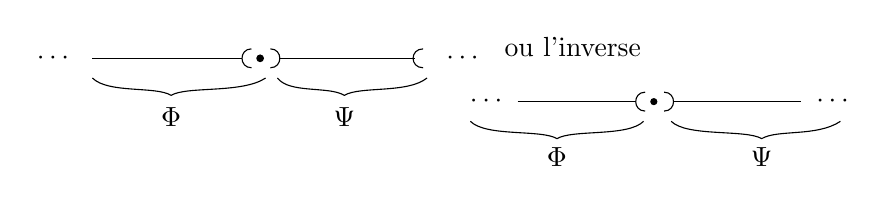
\begin{tikzpicture}[x=1cm,y=1cm]
\node at (-.5,0) {$\cdots$};
\draw (0,0)--(1.9,0);
\draw (2.02,.12) .. controls (1.86,.12) and (1.86,-.12) .. (2.02,-.12);
\fill (2.13,0) circle (1.4pt);
\draw (2.26,.12) .. controls (2.42,.12) and (2.42,-.12) .. (2.26,-.12);
\draw (2.38,0)--(4.1,0);
\draw (4.2,.12) .. controls (4.03,.12) and (4.03,-.12) .. (4.2,-.12);
\draw (0,-.25) .. controls (.2,-.45) and (.8,-.35) .. (1,-.47) .. controls (1.2,-.35) and (1.9,-.45) .. (2.2,-.25);
\draw (2.35,-.25) .. controls (2.5,-.45) and (3,-.35) .. (3.2,-.47) .. controls (3.4,-.35) and (4,-.45) .. (4.25,-.25);
\node at (1,-.75) {$\Phi$};\node at (3.2,-.75) {$\Psi$};
\node at (4.7,0) {$\cdots$};
\node at (6.1,.15) {\unsure{ou l'inverse}};
\node at (5.0,-.55) {$\cdots$};\draw (5.4,-.55)--(6.9,-.55);
\draw (7.02,-.43) .. controls (6.86,-.43) and (6.86,-.67) .. (7.02,-.67);
\fill (7.13,-.55) circle (1.3pt);
\draw (7.26,-.43) .. controls (7.42,-.43) and (7.42,-.67) .. (7.26,-.67);
\draw (7.38,-.55)--(9,-.55);\node at (9.4,-.55) {$\cdots$};
\draw (4.8,-.8) .. controls (5,-1) and (5.7,-.9) .. (5.9,-1.02) .. controls (6.1,-.9) and (6.8,-1) .. (7,-.8);
\draw (7.35,-.8) .. controls (7.55,-1) and (8.3,-.9) .. (8.5,-1.02) .. controls (8.7,-.9) and (9.2,-1) .. (9.5,-.8);
\node at (5.9,-1.25) {$\Phi$};\node at (8.5,-1.25) {$\Psi$};
\end{tikzpicture}}
